%!TEX root = ../TFM.tex


\label{chap:intro} % etiqueta para poder referenciar luego en el texto con ~\ref{sec:intro}

A continuación, se presenta un breve estudio del estado de la Educación de Matemáticas en España actualmente, con el que se pretende ofrecer una visión general del contexto en el que se enmarca este trabajo.


\section{Estado actual de la Educación de Matemáticas en España}
\label{sec:EstadoEducacionMates}

Se tratarán 2 temas fundamentales: la comparativa de España con otros países en la enseñanza de Matemáticas y las actitudes y problemáticas de la educación de Matemáticas en España, más concretamente, los componentes de la actitud de rechazo de algunos estudiantes.


%\paragraph{Informes Internacionales (en Matemáticas)} 

Existen 2 informes internacionales importantes que analizan la competencia matemática: los informes \gls{PISA} y los informes \gls{TIMSS}. 
%
%Para la elaboración de este trabajo se han utilizado exclusivamente los informes \gls{PISA} por varias razones. 
%
Los informes \gls{PISA} se centran en personas de 15 ó 16 años, mientras que, en España, los informes \gls{TIMSS} se están aplicando en 4 E.P.\footnote{El \gls{INEE} así lo especifica en \cite{InformeTimss}.} 
%
Es por ello que los informes \gls{PISA} serán analizados, sobre todo \citePisa{2012;2015}, centrándose el análisis exclusivamente en el apartado de Matemáticas.

En \citePisa{2012} España se sitúa en la posición 33 (de 65) con una puntuación de 484 puntos, siendo esta puntuación inferior a la media OCDE de ese año (494) y a la media UE (489).
%
En el siguiente informe PISA \citePisa{2015}, se produce una mejora en España, siendo la tendencia internacional negativa. 
%
Sin embargo, la puntuación española sigue por debajo de la media internacional.
%
En el cuadro \ref{tbl::ResumenPisa} se encuentran agrupados estos datos.

\begin{table}[hbtp]
\centering
\caption{Resumen de los resultados de los informes \citePisa{2012;2015}}
\label{tbl::ResumenPisa}
\begin{tabular}{c|cccc}
Año & Posición España & Puntuación España & Media OCDE & Media UE\\\hline
2012 & 33 & 484 & 494 & 489\\
2015 & 29 & 486 & 490 & 493
\end{tabular}
\vspace{0.3cm}

\small{Fuente: elaboración propia a partir de los informes \citePisa{2012;2015}.}
\end{table}

No obstante, es importante mencionar que no todas las comunidades autónomas obtienen los mismos resultados. 
%
Por ejemplo, en 2015, algunas comunidades autónomas como Navarra (518), Castilla y León (506), La Rioja (505) y la Comunidad de Madrid (503) se sitúan por encima de la media OCDE.


Otra información relevante aportada por los informes PISA es el porcentaje de estudiantes excelentes -- aquellos que han alcanzado el nivel 5 ó el nivel 6 de las pruebas -- y el porcentaje de estudiantes rezagados -- nivel 1 o inferior --.
%
En la figura \ref{fig::PisaRezEx} se encuentran las gráficas de las tendencias obtenidas en España y en la OCDE según los informes PISA desde 2002.



En el porcentaje de estudiantes rezagados se puede apreciar una ligera mejora en la tendencia española frente a un empeoramiento de la tendencia internacional.
%
A pesar de ello, casi uno de cada 4 adolescentes posee un nivel 1 o inferior de habilidad matemática. 
%
Esta situación es clara e idealmente mejorable.
%
Por otro lado, el porcentaje de estudiantes excelentes en España se mantiene estable en torno al 7\% u 8\% en todos los años, siendo inferior a la media internacional.

Sabiendo cuáles son los resultados obtenidos en España y un marco general de la situación nacional resultaría interesante conocer las causas de esta situación.
%
Debido a que el informe PISA es un informe descriptivo, el trabajo de \cite{ActitudesHaciaMates} será utilizado para descubrir algunos aspectos influyentes en la educación matemática en España.

\begin{figure}[hbt]
\centering
\caption{Porcentaje de estudiantes rezagados (imagen superior) y excelentes (imagen inferior) en España y en los países OCDE. }
\label{fig::PisaRezEx}
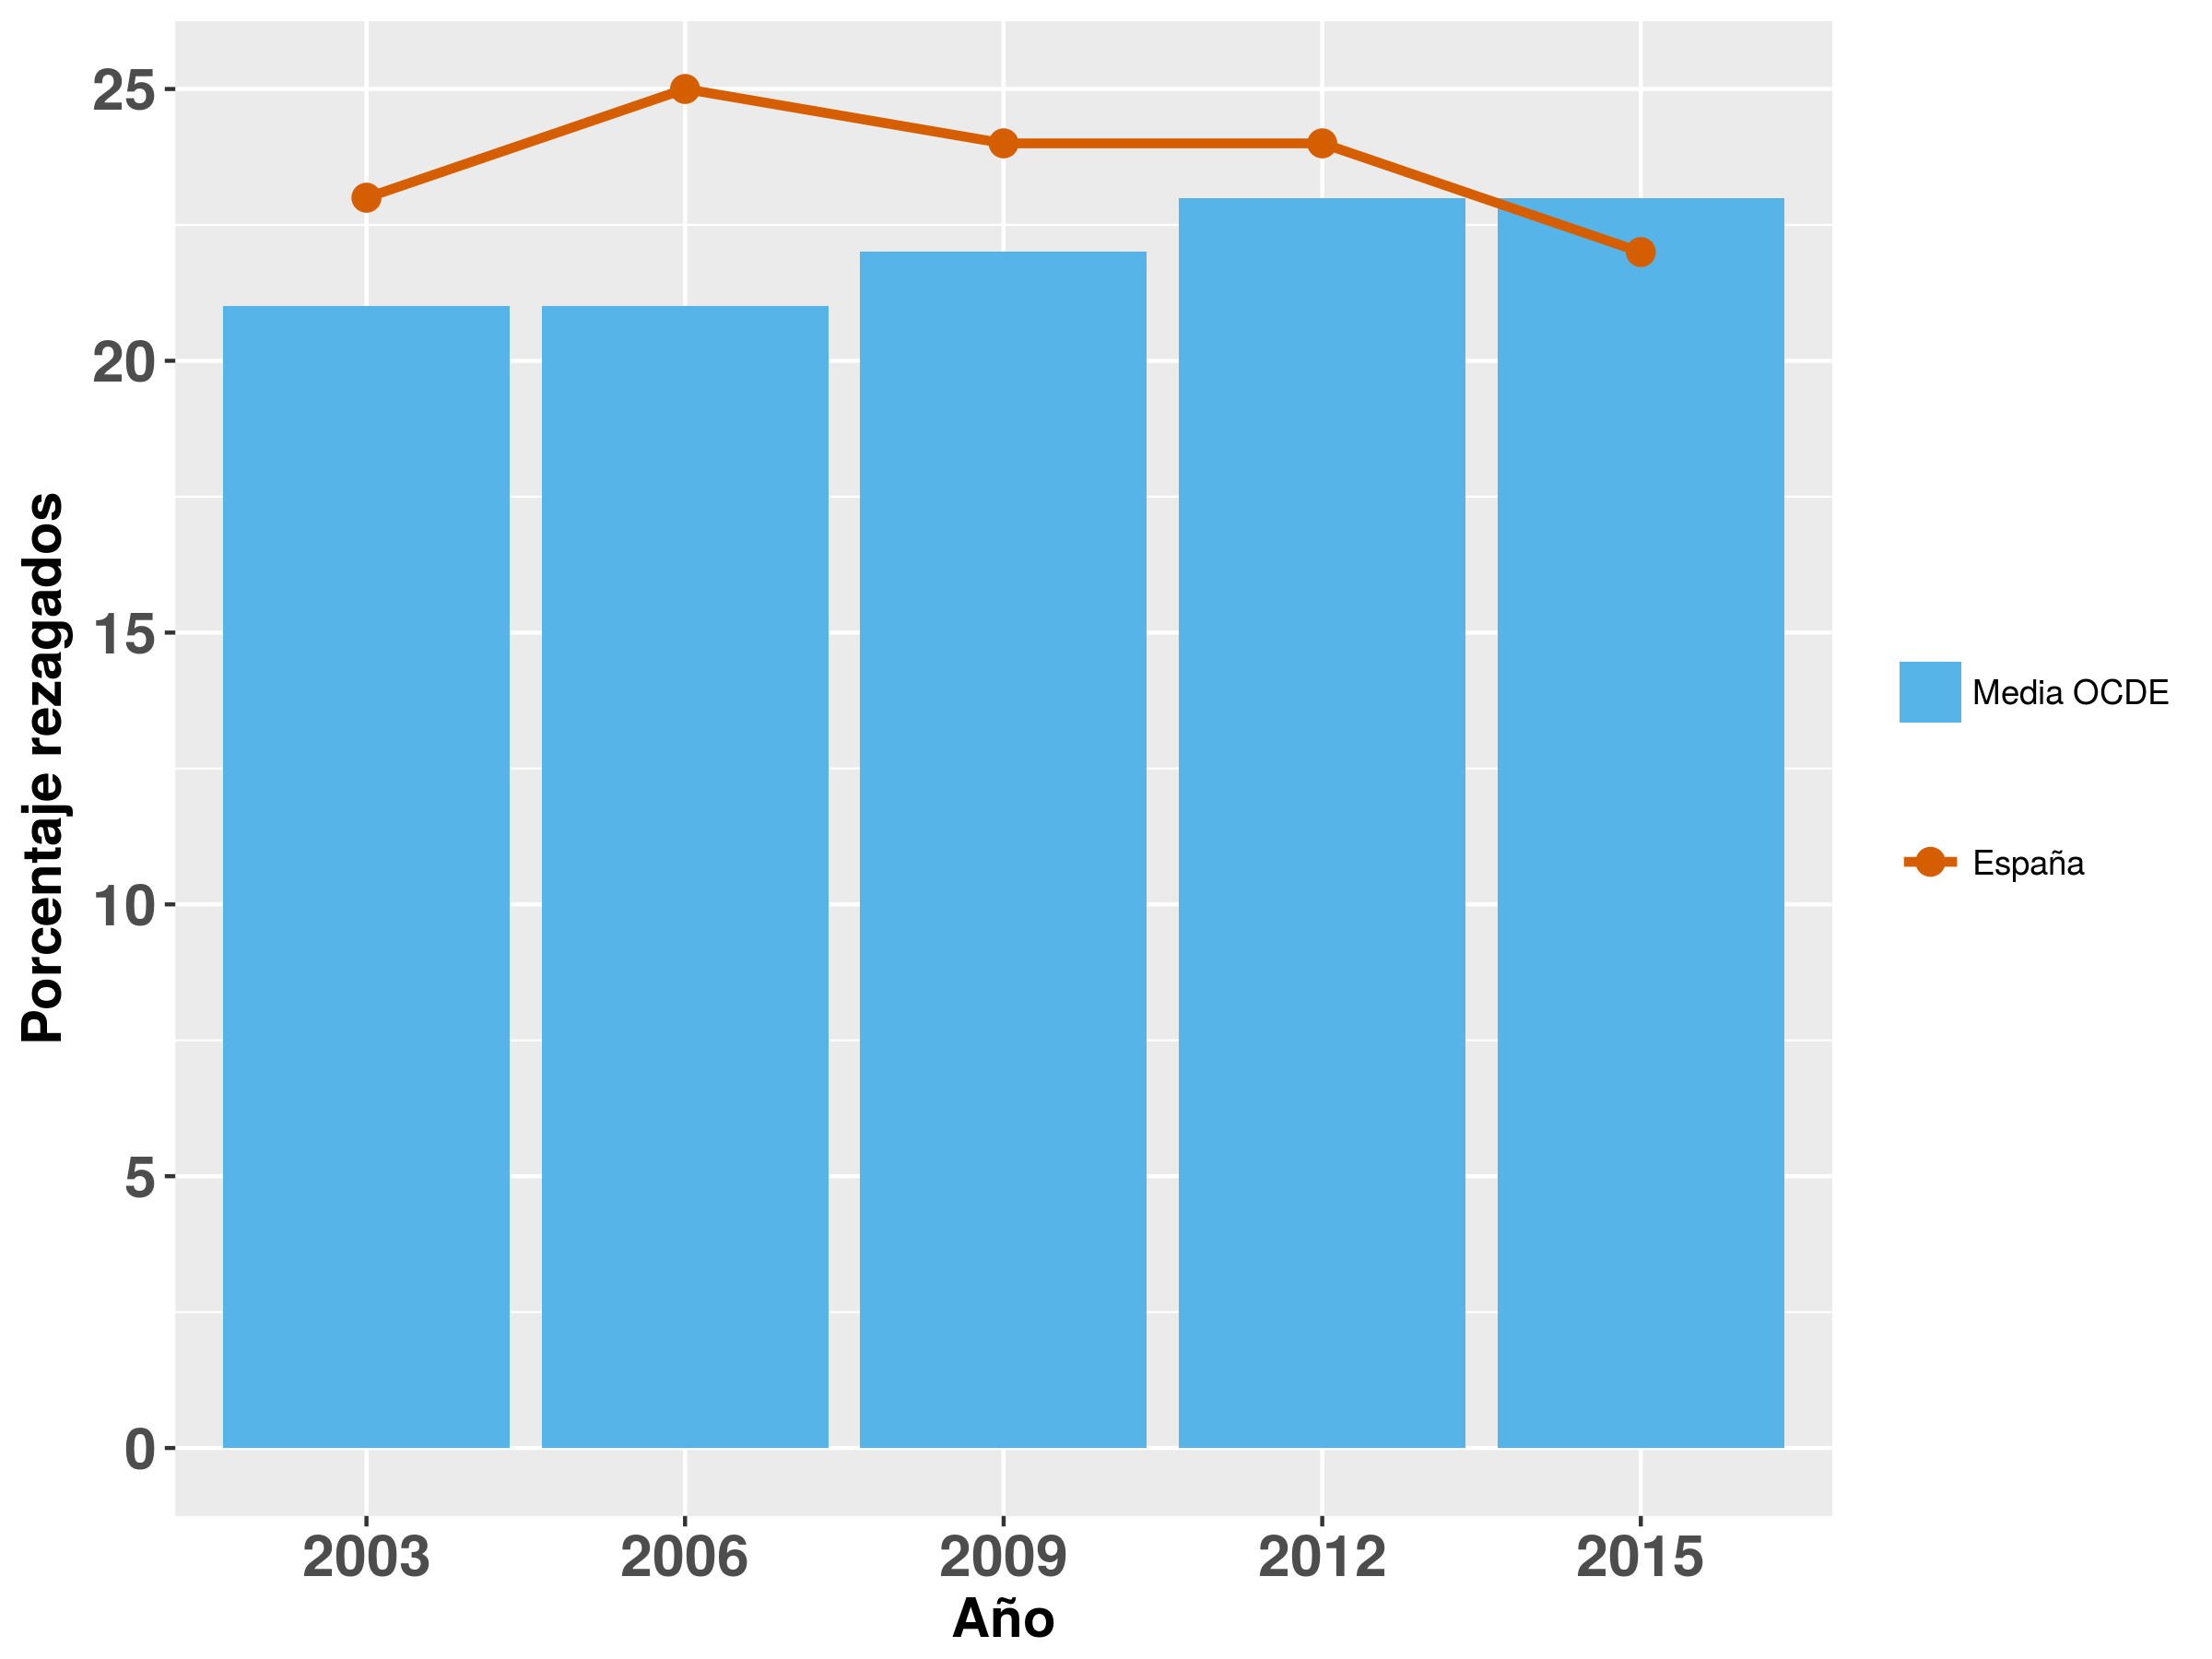
\includegraphics[scale=0.45]{img/PisaRezagados.png}
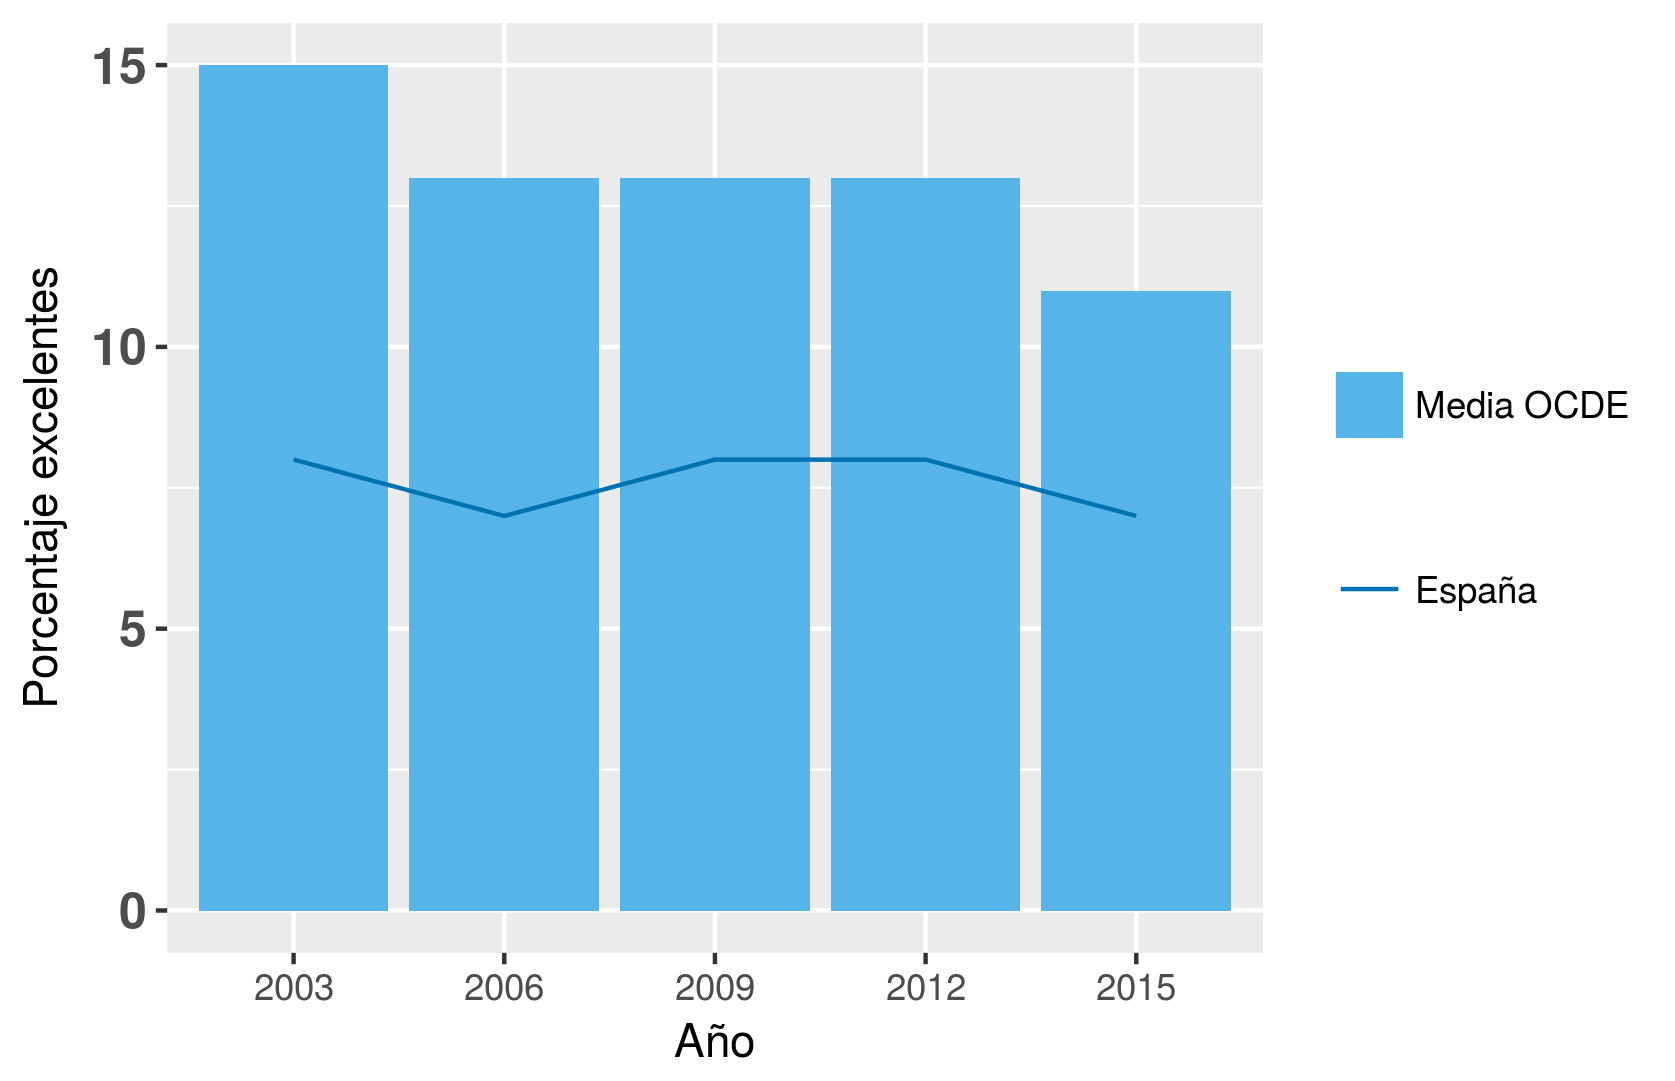
\includegraphics[scale=0.45]{img/PisaExcelentes.png}

\vspace{-0.5cm}
\small{Fuente: Elaboración propia a partir de los informes PISA desde 2002 hasta 2015.}
\end{figure}
\FloatBarrier



%\paragraph{Estudio Nacional}

\label{sec:estudioNacional}
%
\citet*{ActitudesHaciaMates} realizan un estudio transversal para explorar las actitudes hacia las Matemáticas de alumnos en el sistema educativo español, desde tercero de E.P. hasta el primer curso universitario. 
%
Se centra sobre todo en explicar el rechazo de los estudiantes hacia las Matemáticas.
%
El estudio apoya la existencia del siguiente círculo vicioso: 



\begin{figure}[hbt]
\centering
\caption{Circulo vicioso influyente en la actitud de rechazo hacia las Matemáticas según \citep{ActitudesHaciaMates}}
\label{fig::circuloVicioso}
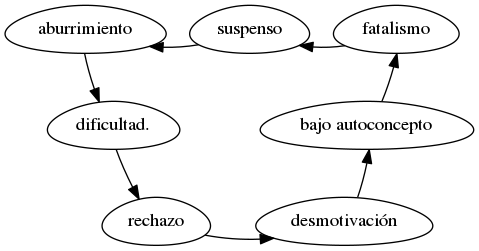
\includegraphics[scale=0.57]{img/circuloVicioso.png}

\small{Fuente: elaboración propia.}
\end{figure}
\FloatBarrier



%El modelo construido utiliza 7 variables (de las 40 estudiadas) 

Al trabajar con una muestra representativa de diversas edades, se puede valorar la influencia de la edad en el rechazo hacia las Matemáticas, comprobándose que el rechazo hacia las Matemáticas aumenta con la edad y las relaciones predictivas se hacen más fuertes.
%
Por ejemplo, el porcentaje de alumnos que rechazan las Matemáticas en 3 de E.P. es del 13.10\%, en 5 E.P. del 28\%  y el de estudiantes de 3 E.S.O. es del 49.50\%.
%
Parece que en la E.S.O. donde se produce un gran aumento del rechazo hacia las Matemáticas.


\cite{ActitudesHaciaMates} estudia 40 variables distintas y construye un modelo 7 variables con un gran poder predictivo 
%
\footnote{El modelo tiene una tasa de acierto en las predicciones del 97\%.}.
%
La variable más influyente del modelo es la percepción de la materia en la escala aburrida-divertida (mayor aburrimiento provoca mayor rechazo), seguida de la percepción de la materia como fácil o difícil (mayor dificultad percibida conlleva mayor rechazo) y de la percepción sobre la autocompetencia para las matemáticas (menor competencia, mayor rechazo).

A estas 3 variables subjetivas e internas del estudiante le sigue la influencia del profesor sobre el rechazo, que se valora si el rechazo hacia las Matemáticas se debe, en cierta medida, a los profesores de Matemáticas que el estudiante ha tenido.
%
La relación es lineal: valores altos de rechazo correlacionan con valores altos de influencia, mientras que valores bajos de rechazo correlacionan con valores bajos de influencia.

La atribución de causalidad de éxito en Matemáticas es otra variable influyente. 
%
Los estudiantes pueden considerar que las aptitudes ejercen una mayor influencia en el desempeño que la dedicación y el estudio, lo cual aumentará el rechazo hacia las matemáticas, ya que creen que no depende tanto de su esfuerzo y dedicación como de su predisposición genética.
%
Asimismo, la competencia percibida para el cálculo mental es también influyente.
%
Por último, la dificultad percibida para el aprendizaje matemático.


Llama la atención que la mayoría de las variables son procesos perceptivos de los estudiantes.
%
Dichas percepciones podrían estar alejadas de la realidad, ya sea por una indefensión aprendida u otros procesos psicológicos.
%
Sin embargo, que sean estas las variables más influyentes ofrece un gran abanico de posibilidades: no parece ser el temario ni la propia disciplina lo más influyente, sino sus percepciones.
%
Una estrategia metodológica diferente podría influir positivamente en algunas de esas percepciones y modificarlas para romper el círculo vicioso.

Asimismo, tras el análisis de la situación de la educación de Matemáticas actual,
%
se ofrece una propuesta metodológica para romper el círculo vicioso (ver \ref{fig::circuloVicioso}), sobretodo en los eslabones de la desmotivación y el aburrimiento.

Si en los cursos de la E.S.O. se consiguiera influir en las percepciones de los estudiantes aparejando Matemáticas y diversión se podrían reducir drásticamente el porcentaje de alumnos rezagados en Matemáticas (ver \ref{fig::PisaRezEx}) y mejorar el nivel matemático general, lo que se reflejaría en los informes internacionales.

